\acresetall
\chapter{Techniques}
\label{ch:intro:techniques}

\section{\textit{In vivo} two-photon Ca\super{2+} imaging}
All of my experiments revolved around two-photon \citep{Denk1990} Ca\super{2+} imaging in hippocampal area CA1 of awake head-fixed mice \citep{Dombeck2007} using genetically-encoded calcium indicators \citep[GECIs,][]{Knopfel2012}, in particular GCaMP6f \citep{Chen2013}.
These methods are based in general on the advances of \citeauthor{Dombeck2007} who established the first awake \textit{in vivo} two-photon recordings in mice and later imaged hippocampal place cells \citep{Dombeck2010}. 
\textit{In vivo} Ca\super{2+} imaging provides several essential advantages over \emph{in vivo} electrophysiological approaches which I made use of in my thesis work.
First, a typical field of view will contain 500-1000 pyramidal cells, allowing me to rapidly collect data from a large number of cells.
This large population sampling was a fundamental part of all of my experiments, but most critical in quantifying the nature of reward enrichment in my \ac{GOL} task (\autoref{sec:df:results:enrichment}) and our work on characterizing the activity of the very low-firing rate \ac{DG} granule cells (\autoref{sec:other:DG}).
Second, actually seeing the cells that I was recording from allowed me to register fields of view from day-to-day and reliably track the same cells for up to 2~weeks.
The main experimental task that I used (\autoref{sec:intro:techniques:GOL}) was a 9-day protocol and tracking the same cells across those 9~days was essential.
A similar protocol was also used in our work characterizing diversity in pyramidal cells along the radial axis of CA1 (\autoref{sec:other:sf-deep}) and this project also critically took advantage of the imaging method by visually identifying superficial and deep CA1 pyramidal cell imaging planes.
Finally, Ca\super{2+} imaging allows for recording activity from cellular compartments other than the soma -- such as dendrites, axons, and even synaptic boutons.
These same recordings are technically very difficult with electrophysiological approaches, and most likely impossible to do over long timescales.
I took advantage of this ability in imaging axons and boutons of \acp{LRIP} from \ac{LEC} to \textit{stratum locunosum-moleculare} in CA1 (see \autoref{sec:other:LRIP}) as our lab has also done in the past \citep{Kaifosh2013, Lovett-Barron2014}.

During my thesis work, the most significant upgrade to our imaging capabilities was the addition of resonant scanning capabilities, which allowed for an up to 10-fold increase in both temporal and spatial resolution, thus greatly improving the quality of our imaging data.
The upgrade also required a corresponding upgrade to our analysis pipeline and server design to handle the significantly increased quantity of data acquired.

\section{Head-fixed behavior}
\label{sec:intro:techniques:behavior}
In order to allow for two-photon Ca\super{2+} imaging in awake mice, I needed to design all behavioral tasks to work while mice are head-fixed under a two-photon microscope (\autoref{fig:intro:techniques:treadmill_schematic}).
Our primary imaging apparatus most directly combines the work of \citeauthor{Dombeck2010} and \citeauthor{Royer2012}.
\citeauthor{Dombeck2010} performed the first two-photon Ca\super{2+} imaging experiments of hippocampal area CA1 place fields and their work provided the basis for our viral GECI strategy and surgery procedure \citep{Dombeck2010}.
\citeauthor{Royer2012} designed a feature-rich head-fixed treadmill for the study of place cells, which was the basis of our original treadmill design \citep{Royer2012}.
While the core apparatus was in place when I began experiments, extensive upgrades were necessary to optimally run my head-fixed learning tasks.
I, along with colleagues in the lab, redesigned the wheels, axles, and platform to minimize friction and facilitate running while head-fixed.
We designed a RFID-tag and quadrature encoding-based system to accurately track position over many laps to within $<$0.5~cm.
We designed new treadmill belts that consist of multiple fabrics sewed together with various cues scattered throughout, which together convey all the spatial information used by mice to anchor place cell maps.
I added features to our in-house behavioral control software to allow for reward schedules that depend on the spatial location of the mouse on the treadmill.
These improvements allowed for the design of new head-fixed behaviors, described below.

\begin{figure}
	\centering
	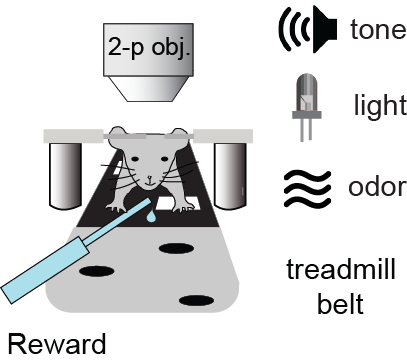
\includegraphics[width=0.5\textwidth]{intro/head_fixed_schematic}
	\caption[Schematic of treadmill design for head-fixed awake two-photon Ca\super{2+} imaging]{Schematic of treadmill design for head-fixed awake two-photon Ca\super{2+} imaging.
	Mice are head-fixed underneath the objective a two-photon microscope (\textsc{2-p obj.}) while they run on a fabric belt consisting of multiple materials with local cues dispersed throughout (\textsc{treadmill belt}).
	Water-deprived mice learn to run for water rewards delivered through a lick port placed in front of them (\textsc{Reward}), which also includes a capacitance sensor to record the timing of each lick (not shown).
	Throughout the task, mice can experience different contextual modes as changes are made to the background, non-spatially-modulated pure tones (\textsc{tone}), blinking colored LED (\textsc{light}), and odors (\textsc{odor}).
	}
	\label{fig:intro:techniques:treadmill_schematic}
\end{figure}

\subsection{Random foraging}
The first task we designed was a simple random foraging task where mice run to get water, but don't need to learn about any particular location on the belt in order to get water rewards.
All head-fixed paradigms begin with 1-2 weeks of training where mice learn to lick for water from a lick port while needing to run progressively farther each session in order to receive another reward (see \autoref{sec:df:methods:training}).
Mice were either operantly rewarded (they must lick to receive water) at random intervals along the belt or non-operantly at a fixed location.
This allowed me to look at baseline stability of spatial maps with two-photon Ca\super{2+} imaging over days or weeks (see \autoref{sec:df:results:rf} \& \autoref{sec:conclusions:chronic}).

\subsection{Goal-oriented learning}
\label{sec:intro:techniques:GOL}
In order to study spatial learning and memory while simultaneously imaging functional activity of hippocampal area CA1 place cells, we developed a head-fixed \acl{GOL} task. The task has been used by me to study spatial memory in a mouse model of \scz/ (\autoref{sec:df:methods:GOL}), by Nathan Danielson to study functional diversity within CA1 pyramidal cells (\autoref{sec:other:sf-deep}), and is now being used by many other people in Attila's lab.
Freely-moving assays of spatial memory in rodents traditionally include the Morris water maze, Barnes maze, or cheese board maze (see \autoref{sec:intro:memory:spatial-reward}).
While head-fixed under a two-photon microscope, mice are constrained to run in effectively a one-dimensional environment (similar to freely moving linear track paradigms) and there are limited options to experimentally assay choices made by the mice.
They key features that we were trying to design in the task were:
\begin{enumerate}
	\item Mice are able to learn a specific rewarded location on the treadmill that is otherwise un-cued.\label{item:into:techniques:GOL:location}
	\item Mice learn the task over several trials to allow for determining a `learning curve'.\label{item:into:techniques:GOL:learning}
	\item A behavioral readout that is sensitive to subtle variations in ability to learn.\label{item:into:techniques:GOL:readout}
	\item Be able to flexibly manipulate the reward and environment parameters to probe mice' ability to learn the task.\label{item:into:techniques:GOL:manip}
\end{enumerate}

Our \ac{GOL} task requires mice to run laps along our multi-fabric, feature-rich circular treadmill belt (for task schematic, see \autoref{fig:df:GOL}).
The mice are water-restricted, so we use water delivered through a lick port as a reward.
Each lap there is one spatial region (\textsc{reward zone}, usually a 20-cm window) on the belt where the mice can operantly receive water rewards: if they lick they get water, if they do not lick, they don't.
The reward will `dry up' after after a fixed amount of time has passed since the mouse entered the reward zone that lap (usually 3 seconds).
Not all mice will run for water rewards at all, and not all mice will perform this task, but many are able to (\ref{item:into:techniques:GOL:location}).
We generally give the mice 9 sessions to learn the reward location.
Some mice will find the reward immediately, but even those that do, they continue to improve and stabilize their performance over the 9 sessions (\ref{item:into:techniques:GOL:learning}).
By measuring the capacitance of the lick port, we can detect changes when the mouse licks, providing us an accurate measure of the time (and the mouse's location on the belt) when each lick occurs.
The operant nature of the reward schedule requires the mice to lick everywhere along the belt to sample each location and find the correct position that will be rewarded.
As the mice learn the reward zone, they suppress licking away from the reward and will then only lick at the reward zone.
We have used multiple measures to quantify this behavior, but generally look at the fraction of licks in the reward zone as a measure of learning (\ref{item:into:techniques:GOL:readout}).
This particular measure can be misleading if the mice lick everywhere along the belt, but then lick robustly once they receive the first drop of water, but in practice we do not see this behavior.
In addition we often look at measures such as \textsc{anticipatory licking}, which quantify the fraction of licks directly preceding the reward, but crucially exclude licks in response to water delivery, though this measure has proven to be less-sensitive to learning.
Finally, the setup allows the experimenter to move the reward to any arbitrary location along the belt, swap out belts to modify the environment, and manipulate non-spatial odor/tone/light cues to change the surrounding context (\ref{item:into:techniques:GOL:manip}).

\section{Data analysis pipeline}
\label{sec:intro:techniques:pipeline}
A typical 10 minute imaging session generates a $\approx$15~GB raw movie that needs to be processed down to a single spatial tuning vector for each of approximately 500 cell somas in the field of view.
Processing each movie requires identifying regions of interest (ROIs), extracting fluorescent signals from each ROI, cleaning up each trace by calculating changes in fluorescence, identifying significant Ca\super{2+} events, aligning Ca\super{2+} event times to the mouses' position in the behavioral environment, and finally calculating place fields for each cell.
Place fields from a single session can tell us how the mice represent the environment in a given session, but to address some of the more interesting questions I wanted to ask how these representations changed over time.
For this, I needed to register ROIs from day-to-day and compare the tuning of the population as a whole over time, but also track changes in the tuning of individual pyramidal cells from session-to-session.
All of these steps need to be performed fast, reliably, and as automatically as possible.
Over the course of my PhD thesis work, I, along with other members of Attila's Lab (especially Patrick Kaifosh and Nathan Danielson), developed a set of programs and tools to complete all of these steps mentioned above.
I will focus here on the pieces that I personally originated or was the primary contributor to, but Attila's lab is collaborative by design and all the code we use is shared, so multiple people have contributed to most aspects of the analysis pipeline.

\begin{figure}
	\centering
	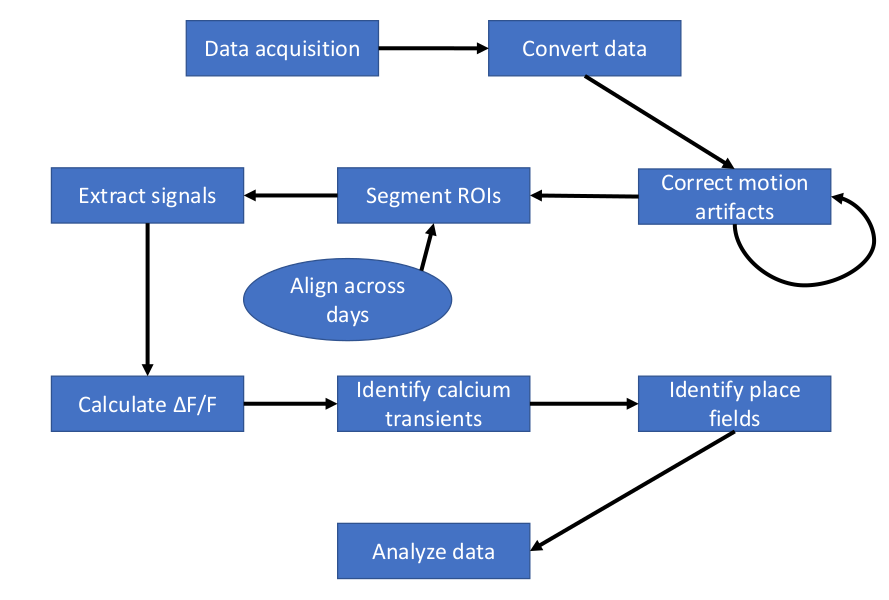
\includegraphics[width=0.9\textwidth]{intro/data_pipeline}
	\caption[Data analysis pipeline]{Data analysis pipeline. Schematic represents the various steps of processing performed on all data.}
	\label{fig:intro:techniques:pipeline}
\end{figure}

\subsection{Initial processing}
\label{sec:intro:techniques:inital}
Imaging data acquired through our microscope software (PraireView) is stored as an individual TIFF image file for every frame of every plane and channel.
This can lead to over 30,000 files per 10 minute recording session, which very quickly becomes difficult to manage.
So, the first step after running an experiment is to move all the data to a special \textsc{scratch} folder on our lab server, where I have a script constantly running to convert all of the data into one large HDF5 file (\url{https://www.hdfgroup.org/HDF5/}).
This format allows us to store all of the data in a 5-dimensional (Time $\times$ Plane $\times$ Row $\times$ Column $\times$ Channel) indexable structure for easy iteration and viewing of the data.
The script checks every individual TIFF file, writes it to the HDF5 file, verifies the integrity of the new HDF5 file, and then moves the new file to a permanent place on the server while deleting the original TIFF files.

At this point the data is now properly formatted for estimation and correction of motion-induced imaging artifacts using our SIMA software package (\autoref{ch:sima}).

% \subsection{Signal extraction}

\subsection{Signal processing}
After signals are extracted for each ROI the next step is to quantify the change in fluorescence over time, as absolute fluorescent values are not interpretable in isolation.
Calculating the change in fluorescent over time is simple in theory: $$\Delta F/F(t) = \frac{F(t) - F_{\circ}}{F_{\circ}},$$ though in practice there are many complications that any algorithm needs to be robust to.
The primary concern is a non-stationary baseline fluorescence, as drift in the baseline intensity can be mistaken for physiological activity, when in fact it is usually due to an experimental artifact.
The most common problem is for the baseline to decay over the course of long recordings, caused by water evaporation/leaking from under the objective, bleaching of the Ca\super{2+} indicator, movement of the tissue out of focus, or some combination of these factors.
While not particularly common, these things do occur and thus need to be accounted for.

Our particular baseline calculation method is based off of \citet{Jia2011}.
In brief, we first smooth the signal with a boxcar smoothing window of width $\tau_1$ and then for every time-point choose the baseline to be the minimum value of this smoothed signal within a $\tau_2$ window.
This effectively implies that there should be a $\tau_1$ size window every $\tau_2$ seconds that is absent of any Ca\super{2+} transients or other large fluctuations.
For hippocampal area CA1 pyramidal cells imaged with GCaMP6f in a well-trained mouse running on a 2-meter long treadmill, we found that $\tau_1$ = 3 seconds and $\tau_2$ = 60 seconds worked well.
As an additional step to aid the robustness of the precise window sizes, we also implemented an iterative procedure where after calculating $\Delta F/F$ we identified significant Ca\super{2+} events (see \autoref{sec:df:methods:transients}) and then re-calculated the $\Delta F/F$ while removing the identified Ca\super{2+} transients from the baseline.
This prevents errors in the baseline calculation for any cells that do not have a 3 second period of quiescence every minute, and was generally repeated 3 times to ensure an accurate baseline calculation.

\subsection{Place cell identification}
\label{sec:intro:techniques:pc_id}
Pyramidal cells in the mammalian hippocampus fire at specific locations within an environment.
% \todo[color=cyan, bordercolor=green, inline]{Add refs and clarify that it is not just familiar but it is thought to be more stable in familiar environments but they are there early on in novel as well with refs. Jeff: this seems beyond this techniques section. I removed 'familiar' and reference the Frank2004 paper on place fields in novel environments.}
We developed an algorithm to reliably identify cells that had a significantly higher mutual information between the mouse's position and the Ca\super{2+} activity of the cell than expected by chance.
The overall goal of our analytical approach is to identify as un-biased a population of spatially-tuned cells as possible.
In particular, we aim to avoid biases in place field width, number of place fields per cell, location of place fields on the belt, or overall cell activity/firing rate level.
In addition, unlike with electrophysiological data, Ca\super{2+} events have a finite duration that we needed to account for on a per-cell basis.  

In brief, we calculate the occupancy normalized transient rate histogram for each cell with bin sizes ranging from 2~cm to 100~cm.
In addition, for each bin size we also rotate the binning through all the possible shifts, such that, for example, if a cell fired transients over any continuous 20~cm segment of the belt, there would be a 20~cm bin that contained all of the transients.

We then calculate the spatial information for each of these bin sizes and bin shifts and take the maximum value as the true spatial information of that cell.
We then shuffle all of the transients within each cell, re-calculate the occupancy normalized transient rate histogram for each bin size and shift as described above, again take the maximum spatial information for this particular shuffle, and then create a distribution of spatial information values across shuffles.
This distribution empirically defines our spatial information confidence threshold for the particular pattern of transient durations and timings for the particular cell.

Additional details of this method can be found in \autoref{sec:df:methods:pc_identification}.
 
\subsection{Lab Analysis Bundle (LAB)}
Over the years, as the lab and our code base grew, the collection of scripts, classes, and functions used for our analysis became hard to mention and difficult for new members to learn.
In order to stabilize the code for future members, I spearheaded an effort to clean-up, refactor, and document all of the code we used in the lab.
This became the Lab Analysis Bundle (LAB), which is a complete Python package hosted privately on GitLab (\url{https://gitlab.com}).
The package is easily installable using standard Python packaging tools, with well-defined dependencies.
As part of refactoring the code, I added automatic documentation to the core functions and standardized the API.
The lab code repository is now in a much more manageable structure that has successfully been passed on to future lab members.

The LAB contains all of the tools needed to analyze behavior and imaging data acquired in Attila's lab.
The core components are:
\begin{itemize}
	\item{Standardized representation of all experimental \textbf{metadata}, including mouse information, experiment start time, and exact behavioral parameters.}
	\item{Scripts for \textbf{processing} of imaging data from raw movies to extracted traces for each ROI.}
	\item{Access to all of the \textbf{behavioral data} acquired during the experiment, such as licking and position information.}
	\item{Object-oriented \textbf{structure} to work with collections of mice and experiments.}
	\item{\textbf{Analysis methods} to calculate behavioral (e.g. fraction of licks near rewards) and functional (e.g. place field correlation) metrics.}
	\item{Generalized \textbf{plotting} functions that work the output of any analysis function.}
	\item{\textbf{Automatic analysis scripts} to quickly perform standard analyses as soon as imaging data is processed.}
\end{itemize}

Below is an example analysis that will plot a histogram of place field widths for all recorded sessions from one mouse.

\begin{lstlisting}[language=Python]
import matplotlib.pyplot as plt
import lab

# Parse experiments metadata
expts = lab.ExperimentSet('behavior_jeff.xml')
# Pull out one particular mouse
mouse = expts.grabMouse('jz119')
# Find all sessions that were imaged
expt_grp = lab.classes.pcExperimentGroup(mouse.imagingExperiments())

# Calculate the width of all place fields
pf_width = lab.analysis.place_cell_analysis.place_field_width(expt_grp)

# Plot a histogram of all the place field widths
ax = plt.axes()
lab.plotting.plot_dataframe(
	ax, [pf_width], plot_method='hist', labels=['jz119'],
	activity_label='Place field width (cm)')

\end{lstlisting}

\begin{figure}[!h]
	\centering
	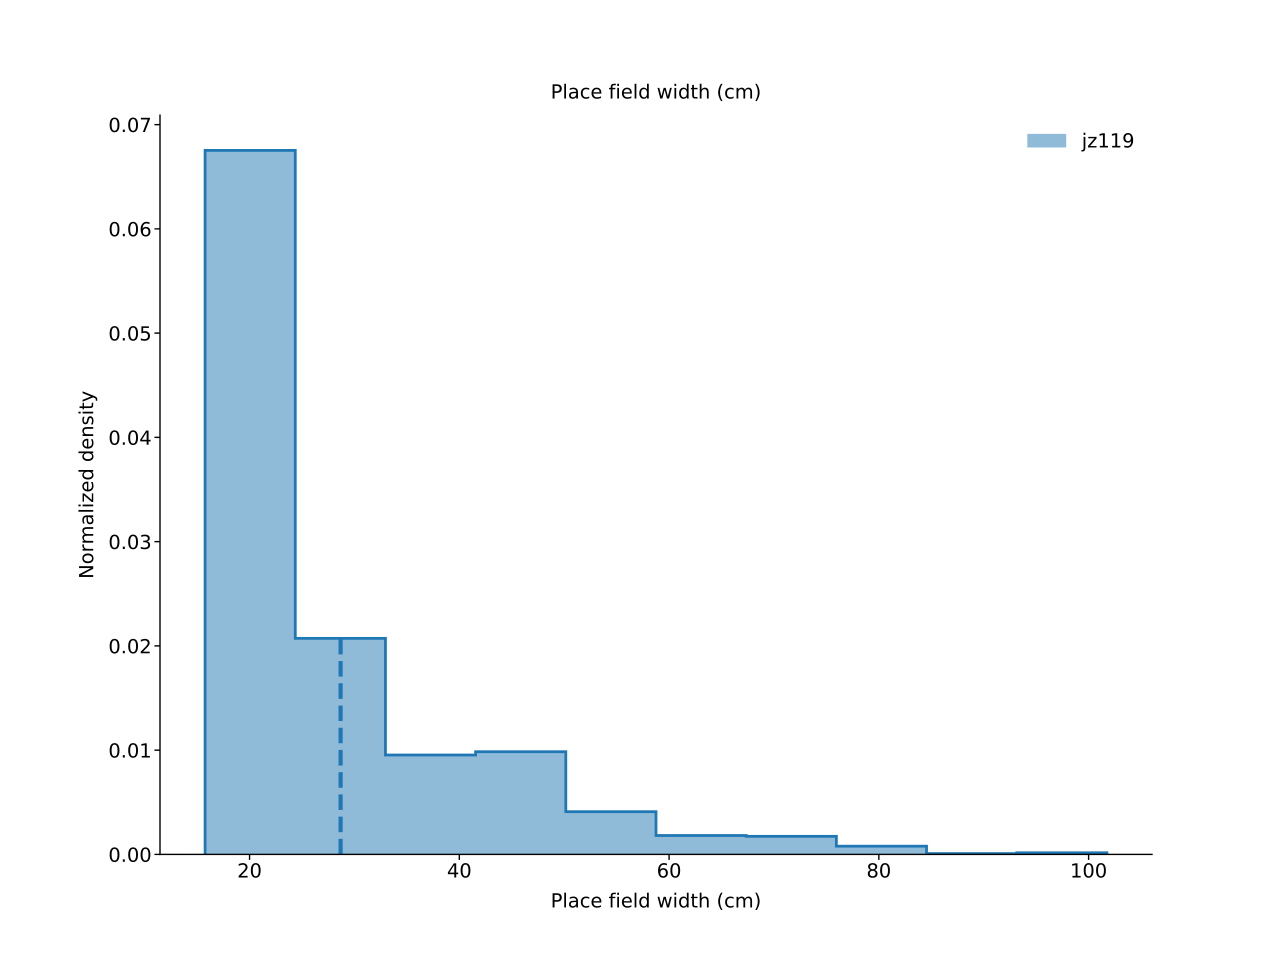
\includegraphics[width=0.7\textwidth]{intro/LAB_pf_width_example}
	\caption[Example histogram]{Example of using LAB to collect experiments, calculate a place cell metric, and plot the data.}
	\label{fig:intro:techniques:pf_width}
\end{figure}


\subsection{Place cell stability}
\label{sec:intro:techniques:stability}
Quantifying the stability of spatial maps is fundamental to most of my thesis work.
There are five commonly used methods for quantifying similarity that I implemented in our analysis package that I will touch on briefly:
\begin{itemize}
	\item{place cell recurrence}
	\item{place field correlation}
	\item{population vector correlation}
	\item{centroid shift}
	\item{firing rate overlap}
\end{itemize}

Place cell \textsc{recurrence probability} is defined between a pair of sessions as the fraction of place cell for the first session that are still identified as place cells in the second session. The null hypothesis that the place cell populations are independent both days would suggest a recurrence probability equal to the fraction of place cells in the second session. This measure captures the stability of the spatially-active population from session-to-session.

\textsc{Place field (PF) correlation} is the correlation between the tuning curve of a cell at two different time points. I subdivided the treadmill belt into 100 evenly-sized bins (each $\approx$2~cm), so every place cell is defined by a 100-element vector of occupancy-normalized Ca\super{2+} transient rates (see \nameref{sec:intro:techniques:pc_id}). The correlation between these vectors gives the place field correlation for that pair of sessions, and these values can be averaged across cells to give a measure of the population stability.
While this is perhaps the most commonly used metric of place cell stability, it is not our preferred measure for quantifying stability of Ca\super{2+} transient-defined place cells.
For Ca\super{2+} data, a perfect place cell will fire a single large transient in the same spatial bin every lap.
This can lead to very spatially-sparse rate maps, as compared to spike-based activity.
Consequently, if the firing location ships very minimally the preferred firing spatial bins may no longer overlap at all, leading to a correlation close to 0, when in fact, the firing has not changed very much.

\textsc{Population vector (PV) correlation} is similar to PF correlation but measures the correlation across cells at each spatial bin, instead of the correlation across spatial bins for each cell.
This metric is calculated by `stacking' place field tuning curves for each cell, and then calculating the correlation between the activity of all the cells at the \textit{same location} from two different sessions.
For my experiments I always binned the data into 100 evenly spaced bins, so for every pair of session I calculate the correlation between 100 population vectors corresponding to each of the 100 spatial bins.
This metric can be used in two separate ways.
First, by averaging across spatial bins we can determine the mean stability of \textit{positions} instead of \textit{cells}, a subtle, but sometimes meaningful distinction.
Also, if we do not average across positions, we can use this measure to look for positions that are specifically more/less stable, such as around the reward location.

\textsc{Centroid shift} is defined per cell as the distance between the center of its place field in two sessions.
We use two separate measures to identify the centroid of a place field.
The first is the more traditional measure, which is the center of mass of transients along the belt.
We define the centroid of each place field separately, so we only use transients that occurred within the place fields when calculating the centroid, and then take the centroid of the place field that had the peak transient rate.
% $$ COM_j = \frac{1}{N}\sum^n_{i=1} m_i r_i,$$
% where $COM_j$ is the center of mass of the $j^{th}$ place field, $N$ is the number of transients, $m_i$ is the weight of each transient 
% \todo[color=green]{Equations for calculating pf centroid?}
In general, I calculated the centroid shift as the absolute value of the distance between the centroids as a fraction of belt, so all values are on $[0, 0.5]$.
An alternative version of the centroid shift ignores place fields and instead represents every transient on the unit circle such that the angle is the position on the circular treadmill and the length is inversely related to the occupancy of that position.
By taking the vector sum of these transient vectors, we can calculate a \textsc{spatial tuning vector}, for each cell for each session (for more details see, \autoref{sec:df:methods:pc_properties}).
Finally, the centroid shift is then defined by the minimum angle between two spatial tuning vectors.
This implementation does not care about place fields, so it is defined for every cell that fires at least 1 transient, which is how I looked at stability of the entire pyramidal cell population.
The main caveat with this measure is that multi-peaked place fields will not be handled correctly, as for example, a place cell with two peaks will have a spatial tuning vector that falls between them.

\textsc{Firing rate overlap} is the similarity of firing rate for a cell between two session. It is simply defined as:
$$\frac{\min{r_1, r_2}}{\max{r_1, r_2}},$$
where $r_1$ and $r_2$ are the firing rates on the first and second session respectively.
This definition means that overlap is defined on $[0, 1]$, with a value of $1$ corresponds to the cell having the same firing rate on both sessions, and a value of $0$ corresponds to a cell that was silent one of the two sessions.
This measure is not defined if the cell was silent both sessions, so those cells were excluded from all analysis.
I generally used transient frequency as a proxy for firing rate, but measures such as the mean of the Ca$^{2+}$ trace or the area under the Ca$^{2+}$ trace during transients worked as well.
